\documentclass[11pt,a4paper]{article}

\usepackage[T1]{fontenc}
\usepackage{lmodern}
\usepackage[margin=2.5cm]{geometry}
\usepackage[numbers,sort&compress]{natbib}
\usepackage[hidelinks]{hyperref}
\usepackage{microtype}
\usepackage{enumitem}
\usepackage{amsmath}
\usepackage{graphicx}
\usepackage{booktabs}
\usepackage{amssymb}
\usepackage{makecell}

\setlength{\parindent}{0pt}
\setlength{\parskip}{0.65em}

\setlist[itemize]{
  leftmargin=1.5em,
  itemsep=0.25em,
  topsep=0.25em
}

\urlstyle{same}

% ---------- Student information ----------
\newcommand{\studentname}{Chengyu Li}
\newcommand{\studentid}{1828290}
\newcommand{\wordcount}{2060}

% ---------- Research topic ----------
\newcommand{\researchtopic}
{Selective Representation Sharing in Multi-Task Recommender Systems}

\newcommand{\researchquestion}
{Under a common backbone and across matched parameter budgets, how does allocating task-specific capacity at the embedding versus expert level affect task-level AUC gains over corresponding single-task baselines, particularly for tasks with sparse positive feedback?}

\title{
  \vspace{-2.2em}
  {\large\textbf{COMP90044 Research Methods}}\\[0.3em]
  {\normalsize Assignment 1 -- Activity 2: Literature Review}\\[0.5em]
  {\LARGE\textbf{\researchtopic}}\\[0.2em]
}

\author{\studentname\quad\studentid}
\date{Word count: \wordcount}

\begin{document}

\maketitle

\vspace{-1.5em}
\begin{center}
\parbox{0.92\textwidth}{
  \small
  \textbf{Research question:} \researchquestion
}
\end{center}
\vspace{0.5em}

\section{Introduction} 
Modern industrial recommender systems often optimise multiple objectives simultaneously. On short-video platforms, user engagement is reflected by signals such as watch time, completion, likes, and shares \citep{cai2024twostage}. Deep multi-task learning architectures have therefore been widely adopted in real-world applications and have achieved strong performance \citep{Ma2018MMoE, wang2025home, Zhang2026SMES}. A common baseline is the shared-bottom architecture, where tasks share lower layers before branching into task-specific towers \citep{Ma2018MMoE}. However, such shared representations can cause negative transfer, where knowledge learned for one task adversely affects the performance of another task \citep{Tang2020PLE}.

To address this issue, one key line of research is the refinement of architecture, known as selective sharing. Instead of sharing all bottom-level parameters unconditionally, these models reserve capacity for individual tasks, extending task-specific components from output towers to gates, experts, and embeddings \citep{Ma2018MMoE, Tang2020PLE, Su2024STEM}. However, greater task-specific capacity can increase parameter, memory, and inference costs, which are tightly constrained in production systems. A separate line of work addresses the same conflict during optimisation rather than through architectural design \citep{Chen2018GradNorm, Yu2020PCGrad, Bai2024GradCraft} and is reviewed here for contrast. This review argues that current evaluations cannot establish where task-specific capacity is best allocated under a fixed parameter budget, because single-task baselines, task-level results, and matched-budget comparisons are rarely reported together.






\section{Shared-Bottom Baseline and Negative Transfer}
\subsection{Shared-Bottom Models}
The baseline model used in this review is the shared-bottom multi-task model. Its underlying principle can be traced back to Rich Caruana \citep{Caruana1997Multitask}, who argued that related tasks can benefit from one another through joint learning of shared representations that capture domain-specific information from the training signals. In modern deep multi-task recommendation, this principle is commonly instantiated through the shared-bottom architecture. As shown in Figure~\ref{fig:architectures}(a), this architecture contains several hidden layers following the input layer that are shared across all tasks. A task-specific tower is then built on top of the resulting shared representation for each task \citep{Ma2018MMoE}. 

Given $K$ tasks, the output of task $k$ can be formulated as
\begin{equation}
    y_k = h^k(f(x)),
    \label{eq:shared-bottom}
\end{equation}
where $f(\cdot)$ denotes the shared-bottom network and
$h^k(\cdot)$ denotes the task-specific tower for task $k$.

\begin{figure}[htbp]
\centering
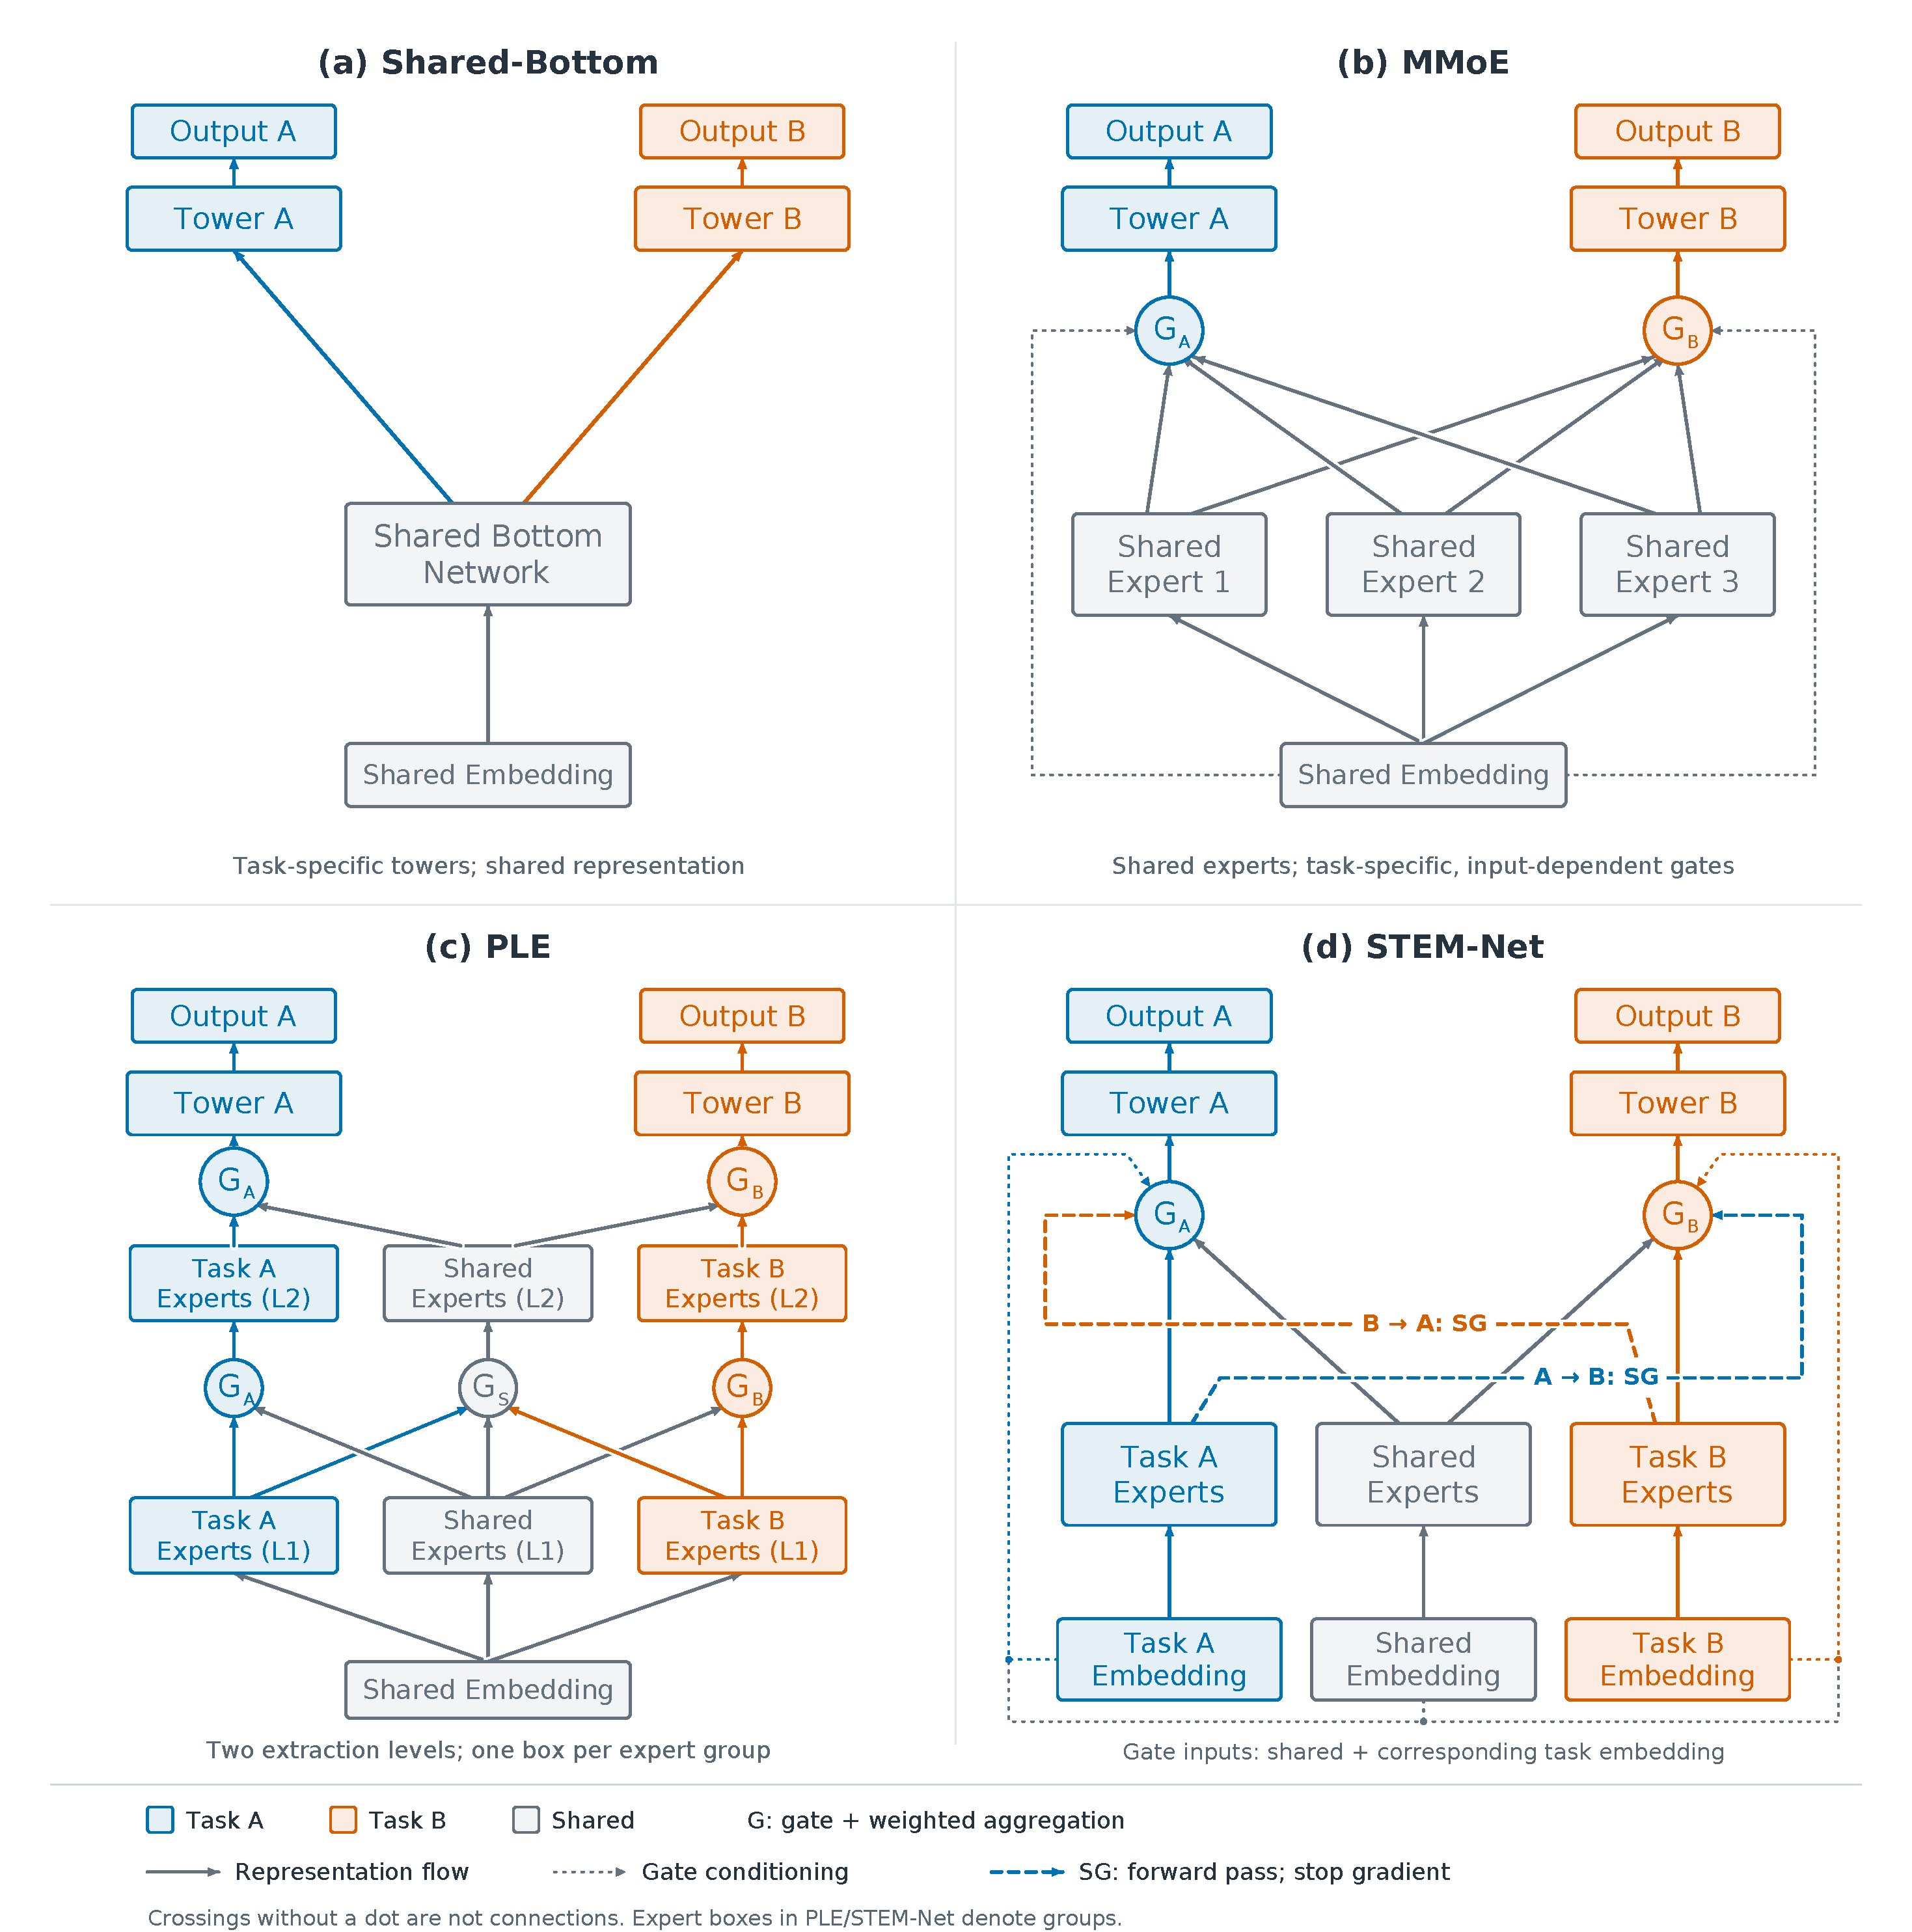
\includegraphics[height=0.62\textheight,keepaspectratio]{mtl_architectures.pdf}
\caption{Selective sharing architectures. Task-specific capacity moves from towers (a) to gates (b), experts (c), and embeddings (d). Line crossings without a junction dot do not indicate connections.}
\label{fig:architectures}
\end{figure}

\subsection{Negative Transfer}
\citet{BenDavid2008TaskRelatedness} theoretically formalised task relatedness as a key condition for the potential benefits of multitask learning (MTL). When task objectives are only partially aligned, sharing across tasks without accounting for their relatedness may lead to performance degradation, a phenomenon known as negative transfer \citep{pmlr-v48-leeb16, Wang2019NegativeTransfer}. Negative transfer in MTL can be explained through two important mechanisms. The first mechanism arises from gradient conflict, where different tasks generate conflicting or even opposing gradient directions when updating shared parameters, characterised by negative cosine similarity \citep{Yu2020PCGrad}. Another mechanism arises from gradient magnitude imbalance, where some tasks may generate substantially larger backpropagated gradients than others. This imbalance can cause certain tasks to dominate the updates of shared parameters, consequently distorting the joint optimisation process \citep{Chen2018GradNorm}. In the shared-bottom architecture, since all tasks share the same shared-bottom parameters under a fixed sharing structure regardless of task relatedness, the model may suffer from optimisation conflicts caused by task differences \citep{Ma2018MMoE}. 






\section{Architectural Evolution toward Selective Representation Sharing}

% \subsection{Cross-Stitch Networks}
% Cross-Stitch shifted the degree of representation sharing from a manually
% specified design choice to a learnable component of the model. As shown in
% Figure~\ref{fig:cross-stitch}, given task-specific representations $x_A$ and
% $x_B$, a cross-stitch unit learns the degree of representation sharing through
% linear combinations $\tilde{x}_A$ and $\tilde{x}_B$:
% \begin{equation}
% \begin{bmatrix}
% \tilde{x}_A \\
% \tilde{x}_B
% \end{bmatrix}
% =
% \begin{bmatrix}
% \alpha_{AA} & \alpha_{AB} \\
% \alpha_{BA} & \alpha_{BB}
% \end{bmatrix}
% \begin{bmatrix}
% x_A \\
% x_B
% \end{bmatrix},
% \label{eq:cross-stitch}
% \end{equation}
% where the resulting representations are fed into subsequent task-specific
% layers \citep{Misra2016CrossStitch}.

% Despite its limited sample adaptivity due to static mixing weights shared
% across samples \citep{Tang2020PLE}, and the additional parameter cost
% associated with maintaining task-specific network streams
% \citep{Ma2018MMoE}, Cross-Stitch provided an architectural insight relevant
% to multi-objective recommendation: representation sharing need not be
% architecturally fixed or binary, but can instead be learned while preserving
% task-specific representations.


% \begin{figure}[t]
%     \centering
%     \fbox{
%         \parbox[c][4.5cm][c]{0.85\linewidth}{
%             \centering
%             Placeholder for Figure 2\\[0.5em]
%             Cross-Stitch Network\\[0.5em]
%             Two task-specific streams with learnable\\
%             cross-task representation mixing
%         }
%     }
%     \caption{Conceptual illustration of the Cross-Stitch architecture, where task-specific representations are selectively mixed through learnable cross-stitch units.}
%     \label{fig:cross-stitch}
% \end{figure}


\subsection{Multi-gate Mixture-of-Experts (MMoE)}

Building on the shared-bottom model, MMoE has become a representative architecture for industrial multi-task recommendation \citep{Ma2018MMoE}. Figure~\ref{fig:architectures}(b) illustrates the architecture, which retains a task-specific tower for each task, with the prediction for task $k$ given by

\begin{equation}
y_k = h^k\left(f^k(x)\right),
\label{eq}
\end{equation}

where $h^k(\cdot)$ denotes the task-specific tower and $f^k(x)$ is the representation supplied to it. Rather than producing this representation through a single shared-bottom network, MMoE combines a pool of shared experts:

\begin{equation}
f^k(x)
=
\sum_{i=1}^{n} g_i^k(x)f_i(x),
\label{eq}
\end{equation}

where $f_i(x)$ is the output of expert $i$ and $g_i^k(x)$ is its weight for task $k$. These weights are generated by an input-dependent, task-specific gate:

\begin{equation}
g^k(x)
=
\operatorname{softmax}\left(W_{gk}x\right).
\label{eq}
\end{equation}

MMoE therefore introduces task-specific selection at the gate level, allowing each task to form input-dependent expert mixtures while keeping all expert parameters shared. In the original experiments, MMoE showed its clearest advantage over baselines when tasks were weakly related and also improved performance in large-scale content recommendation \citep{Ma2018MMoE}. However, insufficient differentiation among shared experts may still produce the seesaw phenomenon, in which improvement in one task accompanies degradation in another \citep{Tang2020PLE}. This limitation motivates PLE to introduce task-specific experts.

\subsection{Progressive Layered Extraction (PLE)}
To address the limited expert differentiation in MMoE, PLE explicitly separates shared and task-specific experts \citep{Tang2020PLE}. As Figure~\ref{fig:architectures}(c) shows, a task-specific gate at each extraction layer combines its corresponding task-specific experts with the shared experts, while a shared gate aggregates information from all experts for the next layer. Stacking these extraction modules progressively separates shared and task-specific representations. For task $k$, the output of its gate at extraction layer $j$ is

\begin{equation}
g^{k,j}(x)
=
w^{k,j}\left(g^{k,j-1}(x)\right)S^{k,j}(x),
\label{eq}
\end{equation}

where $w^{k,j}(\cdot)$ produces gate weights from the previous-layer representation and $S^{k,j}(x)$ contains the expert outputs available to task $k$ at layer $j$. Experiments on large-scale video recommendation data show that PLE outperforms MMoE across different task relationships and task-group sizes \citep{Tang2020PLE}. However, PLE retains shared embeddings, which may obscure task-specific user preferences \citep{Su2024STEM}. Moreover, adding a task requires additional task-specific experts, gates, and a tower, causing task-specific capacity to grow with the number of tasks. 


% \subsection{Shared and Task-specific Embeddings (STEM)}
% To address this limitation, STEM incorporates shared and
% task-specific embeddings to capture both common and
% task-specific user preferences \citep{Su2024STEM}.
% As illustrated in Figure~\ref{fig:stem}, STEM-Net allows
% each task tower to receive outputs from shared and all
% task-specific experts, while blocking gradients through
% other tasks' expert outputs. The representation for task
% $t$ is computed as
% \begin{equation}
% \begin{aligned}
% o^t ={}&
% \sum_{i=1}^{K_1} g_i^{t\to t}h_i^t
% +
% \sum_{j=1}^{K_2} g_j^{S\to t}h_j^S \\
% &+
% \sum_{\substack{t'=1 \\ t'\neq t}}^{T}
% \sum_{i=1}^{K_1}
% g_i^{t'\to t}\operatorname{SG}(h_i^{t'}),
% \end{aligned}
% \label{eq:stem-gating}
% \end{equation}
% where $h$ denotes expert outputs and $g$ denotes gating
% weights. Each of the $T$ tasks has $K_1$ task-specific
% experts, alongside $K_2$ shared experts.
% The stop-gradient operator $\operatorname{SG}$ preserves
% outputs in the forward pass but blocks gradients in
% backpropagation, enabling cross-task knowledge transfer
% while protecting task-specific experts and embeddings
% from updates by other tasks.

% In their experiments, STEM-Net outperforms PLE in average AUC across all three datasets and achieves positive transfer relative to single-task models on the Like task in both TikTok and QK-Video, supporting the effectiveness of its selective-sharing design.


\subsection{Shared and Task-specific Embeddings (STEM)}
To address the shared-embedding limitation retained by PLE, STEM introduces one shared embedding table and a separate embedding table for each task, enabling common and task-specific user preferences to be represented separately \citep{Su2024STEM}. Shared experts receive the shared embeddings, whereas each task-specific expert group receives embeddings from its corresponding task-specific table. As illustrated in Figure~\ref{fig:architectures}(d), each task tower then aggregates outputs from its own task-specific experts, the shared experts, and the other tasks' experts, weighted by gates computed from both shared and task-specific embeddings. Outputs from the other tasks' experts are passed through a stop-gradient operator, which preserves them in the forward pass but blocks their gradients, enabling direct cross-task transfer while protecting task-specific parameters from updates by other tasks.

STEM-Net outperforms PLE in average AUC across all three datasets and achieves positive transfer over the corresponding single-task baselines on the low-positive-rate Like task in both TikTok and QK-Video \citep{Su2024STEM}. However, assigning task-specific embeddings to additional feature fields can substantially increase parameter count, motivating the capacity-allocation question examined later.

% As illustrated in Figure~\ref{fig:architectures}(d), each task tower then receives outputs from the shared and all task-specific experts. The representation for task $t$ is

% \begin{equation}
% \begin{aligned}
% o^t ={}&
% \sum_{i=1}^{K_1} g_i^{t\to t}h_i^t
% +
% \sum_{j=1}^{K_2} g_j^{S\to t}h_j^S \
% &+
% \sum_{\substack{t'=1 \ t'\neq t}}^{T}
% \sum_{i=1}^{K_1}
% g_i^{t'\to t}\operatorname{SG}(h_i^{t'}),
% \end{aligned}
% \label{eq:stem-gating}
% \end{equation}

% where $h$ denotes expert outputs and $g$ denotes gating weights computed from both shared and task-specific embeddings. Each of the $T$ tasks has $K_1$ task-specific experts, alongside $K_2$ shared experts. The stop-gradient operator SG preserves other tasks' expert outputs in the forward pass but blocks their gradients, enabling direct cross-task transfer while protecting task-specific parameters from updates by other tasks.

\subsection{Recent Diversification of Selective Sharing}
The progression above assumes that task-specific capacity, once added, can be effectively trained and served at acceptable cost.
HoME \citep{wang2025home} identifies expert collapse, degradation, and underfitting,
showing that data-sparse tasks—precisely those that motivate task-specific capacity—may
fail to utilise their own experts. MoME \citep{Xu2024MoME} and SMES \citep{Zhang2026SMES}
instead question its cost, reducing storage redundancy through masked expert
subnetworks and limiting the experts executed at inference through sparse routing.
Because these studies optimise different efficiency measures, existing results do not
establish which placement of task-specific capacity best preserves task-level positive
transfer under comparable parameter budgets.





\section{Optimisation-Based Approaches to Negative Transfer}

Architectural methods determine what is shared and where, but shared parameters may still receive conflicting or imbalanced task gradients. GradNorm \citep{Chen2018GradNorm} dynamically adjusts task-loss weights to balance gradient magnitudes and training rates, whereas PCGrad \citep{Yu2020PCGrad} removes gradient components that conflict in direction before aggregation. GradCraft \citep{Bai2024GradCraft} combines both strategies by balancing gradient magnitudes and projecting each gradient against all conflicting tasks. These methods complement selective-sharing architectures by controlling how shared parameters are updated rather than where task-specific capacity is allocated. However, because they do not add model capacity, they leave the parameter and inference costs of task-specific embeddings and experts unchanged; they can therefore be applied under a fixed parameter budget, but cannot substitute for decisions about where task-specific capacity is placed.

\section{Comparative Evidence and Remaining Limitations}

\subsection{Task-Level Benefits and Positive Transfer}
Recent multi-task recommendation methods frequently report improvements over prior state-of-the-art models in terms of average AUC. However, average performance may conceal substantial variation in task-level transfer, including performance degradation on individual tasks. Therefore, a more informative task-level measure, $\Delta \mathrm{AUC}_t$, can be defined as the AUC gain of a multi-task model relative to its corresponding single-task baseline:

\begin{equation}
\Delta \mathrm{AUC}_t
=
\mathrm{AUC}_t^{\mathrm{MTL}}
-
\mathrm{AUC}_t^{\mathrm{STL}}.
\end{equation}

A positive value indicates positive transfer, whereas a negative value indicates that multi-task learning harms the performance of task $t$. Applying this measure to the KuaiRand1K results reported by STEM \citep{Su2024STEM} gives the task-level gains shown in Table~\ref{tab:stem_task_gain}. Tasks C, E, and F have positive-feedback rates of 0.10\%, 0.08\%, and 0.10\%, respectively, making them the three sparsest tasks by positive-feedback rate. They also achieve the largest AUC gains of $+0.0126$, $+0.0063$, and $+0.0249$. In contrast, Task D remains highly sparse at 0.26\% but shows a negative gain of $-0.0033$. Moreover, the two densest tasks, A and G, also experience small performance declines. Overall, the benefits of STEM are concentrated among the sparsest tasks, but the relationship between positive-feedback sparsity and task-level gain is not monotonic. Therefore, sparsity alone does not guarantee positive transfer. The reported results lack run-to-run variance estimates, so small task-level differences should be interpreted cautiously.

\begin{table}[htbp]
\centering
\caption{Task-level AUC gains of STEM-Net relative to single-task models on KuaiRand1K.}
\label{tab:stem_task_gain}
\resizebox{\columnwidth}{!}{
\begin{tabular}{ccccc}
\hline
\textbf{Task} &
\textbf{Positive Ratio} &
\textbf{STEM-Net AUC} &
\textbf{Single-Task AUC} &
$\boldsymbol{\Delta\mathrm{AUC}_t}$ \\
\hline
A & 37.76\% & 0.7523 & 0.7534 & $-0.0011$ \\
B & 1.54\%  & 0.9282 & 0.9293 & $-0.0011$ \\
C & 0.10\%  & 0.8420 & 0.8294 & $\mathbf{+0.0126}$ \\
D & 0.26\%  & 0.8910 & 0.8943 & $-0.0033$ \\
E & 0.08\%  & 0.8635 & 0.8572 & $\mathbf{+0.0063}$ \\
F & 0.10\%  & 0.9070 & 0.8821 & $\mathbf{+0.0249}$ \\
G & 26.17\% & 0.7637 & 0.7650 & $-0.0013$ \\
H & 1.78\%  & 0.8359 & 0.8358 & $+0.0001$ \\
\hline
\end{tabular}
}
\end{table}

A similar pattern can be observed in the MMLRec benchmark \citep{yuan2024mmlrec}. On KuaiRec, PLE improves the average AUC from 0.7214 to 0.7240 ($+0.0026$). However, its AUC on Task 1 decreases from 0.7352 to 0.7328 ($-0.0024$), while that on Task 2 increases from 0.7077 to 0.7152 ($+0.0075$). Hence, the average gain conceals the performance degradation on Task 1, further demonstrating that average AUC cannot indicate whether every task benefits from multi-task learning.


% \subsection{Resource Costs and Comparability}
% Industrial deployment imposes latency and memory constraints, so resource cost determines whether a predictive gain can be used at all. Efficiency is widely reported in this line of work, but not consistently measured. As reported by STEM \citep{Su2024STEM}, STEM-Net achieves an AUC of 0.8301 on TikTok using only user-side features with 1.23$\times$ the number of parameters, while the all-feature configuration increases the parameter count to 2.85$\times$ but achieves only a marginally higher AUC of 0.8304. In contrast, the item-side configuration uses 2.62$\times$ the parameters but achieves an AUC of 0.8260, offering no improvement over the variant without task-specific embeddings. A similar pattern appears on KuaiRand1K, where the item-side configuration reduces AUC from 0.8382 to 0.8193. These results suggest that additional task-specific capacity does not necessarily improve performance, and that how this capacity is allocated across the model may matter more than simply increasing the parameter count. MoME instead reports model size in MB, with a substantial part of the reduction arising from storing binary masks at one bit per parameter rather than the 32 bits typically required by experts in MoE-based models \citep{Xu2024MoME}. However, storage efficiency is not equivalent to computational efficiency: the paper does not report latency or FLOPs, making it difficult to determine how far the reported memory savings translate into reduced inference cost. SMES reports both total parameter count and inference latency, showing that these measures can diverge. When scaled to 0.6B parameters, SMES achieves an average GAUC improvement of 0.84\% while increasing latency by only 4\,ms, whereas dense models exhibit approximately linear latency growth as their parameter counts increase \citep{Zhang2026SMES}. This occurs because sparse routing limits the number of experts activated for each instance. Consequently, total parameter count is an incomplete proxy for the inference cost of sparsely activated architectures. MGOE provides further evidence that efficiency cannot be characterised by a single metric. On Taobao, PLE and STEM have comparable parameter counts, at 13.29M and 13.59M respectively, yet their training times differ markedly, at 957s and 438s. More strikingly, although MMoE uses fewer parameters and less GPU memory than MGOE, it still requires longer training time, 333s compared with 258s \citep{Yao2026MGOE}. Parameter efficiency, memory efficiency, and runtime efficiency therefore do not necessarily align, and model rankings can reverse depending on which cost is measured.

\subsection{Resource Costs and Comparability}
Industrial deployment imposes latency and memory constraints, making resource cost central to whether predictive gains are practically usable. However, efficiency is measured inconsistently across multi-task recommendation studies. STEM's field ablation shows that parameter growth does not reliably predict performance. On KuaiRand1K, item-side specialisation uses 2.05$\times$ the parameters of the baseline configuration yet reduces average AUC from 0.8382 to 0.8193 \citep{Su2024STEM}. Since field coverage and capacity change together, this experiment cannot isolate either effect; nevertheless, it shows that parameter count alone cannot explain performance and motivates examining where task-specific capacity is allocated.


MoME instead measures model size in MB, largely benefiting from one-bit binary masks, but does not report FLOPs or latency \citep{Xu2024MoME}. Its storage savings therefore cannot be directly interpreted as reduced inference cost. SMES further shows that total parameters and latency can diverge: scaling to 0.6B parameters improves average GAUC by 0.84\% while adding only 4\,ms of latency because only a bounded number of experts are activated per instance \citep{Zhang2026SMES}.

MGOE similarly demonstrates that cost measures can produce different model rankings. PLE and STEM have comparable parameter counts, at 13.29M and 13.59M, but require 957s and 438s of training time, respectively. MMoE uses fewer parameters and less GPU memory than MGOE, yet takes longer to train, at 333s versus 258s \citep{Yao2026MGOE}. Even MMLRec, a unified benchmark for multi-task recommendation, standardises datasets, preprocessing, and predictive evaluation but reports only training time per epoch among its resource measures \citep{yuan2024mmlrec}. Consequently, parameter count, storage, memory, training time, and inference latency cannot be treated as interchangeable measures or used to construct directly comparable efficiency rankings.
 


\subsection{Limits of Existing Evaluation}
Answering the research question requires an evaluation that tracks task-level gains over single-task baselines across multiple matched parameter budgets while controlling where task-specific capacity is placed. Table~\ref{tab:evaluation_evidence} summarises the available evidence. STEM and MoME provide single-task baselines, but their capacity ablations primarily report average AUC \citep{Su2024STEM, Xu2024MoME}. HoME and SMES report task-level results under capacity changes, but omit corresponding single-task baselines; moreover, SMES matches architectures at only one budget point \citep{wang2025home, Zhang2026SMES}. OneRank scales encoder depth and width, but measures gains relative to its smallest configuration rather than to single-task models \citep{Tang2026OneRank}, while MGOE evaluates only one differently sized configuration per architecture \citep{Yao2026MGOE}. Consequently, the reviewed studies do not combine task-level gains over single-task baselines, multiple matched budgets, and a controlled comparison of embedding- and expert-level capacity. Since PLE and STEM differ in gating and gradient flow, directly comparing their original implementations cannot isolate the effect of capacity placement.

% 需要 \usepackage{booktabs} 和 \usepackage{makecell}
\begin{table}[!t]
\centering
\small
\caption{Evidence provided by capacity-related evaluations in the reviewed studies.
STL baselines in STEM, MoME, OneRank, and MGOE are reported outside their capacity
analyses. OneRank's scaling gains are measured relative to its smallest configuration
rather than to single-task models.}
\label{tab:evaluation_evidence}

\begin{tabular}{lcccl}
\toprule
\textbf{Study}
& \makecell{\textbf{Per-task results under}\\\textbf{capacity change}}
& \makecell{\textbf{STL}\\\textbf{baseline}}
& \makecell{\textbf{Multiple matched}\\\textbf{budgets}}
& \textbf{Capacity varied at} \\
\midrule

STEM \citep{Su2024STEM}
& No (average only)
& Yes
& No
& Embedding fields \\

MoME \citep{Xu2024MoME}
& No (average only)
& Yes
& No
& Expert masking/pruning \\

HoME \citep{wang2025home}
& Yes
& No
& No
& Expert number \\

SMES \citep{Zhang2026SMES}
& Yes
& No
& No (one point)
& Expert sparse routing \\

OneRank \citep{Tang2026OneRank}
& Yes
& Yes
& No
& Encoder depth/width \\

MGOE \citep{Yao2026MGOE}
& No sweep
& Yes
& No
& --- \\

\bottomrule
\end{tabular}
\end{table}



\section{Research Gap and Future Direction}
The evidence reviewed above shows that improvements in average performance can coexist
with negative transfer on individual tasks. It also demonstrates that parameter count,
storage, memory consumption, and runtime capture distinct aspects of resource cost.
Neither observation, however, has been brought to bear on where task-specific capacity should be placed when models are compared under matched parameter budgets. This motivates the following research question:

\begin{quote}
\begin{minipage}{\linewidth}\itshape
\textit{Under a common backbone and across matched parameter budgets, how does allocating task-specific capacity at the embedding versus expert level affect task-level AUC gains over corresponding single-task baselines, particularly for tasks with sparse positive feedback?}
\end{minipage}
\end{quote}

A suitable evaluation would construct embedding-specialised and expert-specialised variants under a common backbone and match their total trainable parameter counts at several budget levels. Each variant would be compared with corresponding single-task baselines using $\Delta\mathrm{AUC}_t$. Parameter count would serve as the controlled quantity, with memory consumption and inference latency reported as complementary resource measures. This evaluation would reveal whether positive transfer for sparse tasks is preserved as capacity becomes constrained and distinguish the effect of capacity placement from that of simply increasing model size.


% \nocite{*}

\newpage
\bibliographystyle{IEEEtranSN}
\bibliography{references}

\newpage
\appendix
\section{GenAI Usage}

GenAI was used as a supporting tool during the preparation of this literature review. Representative uses included improving grammar, clarity, concision, and academic phrasing; discussing papers that had already been read; checking calculations and values used in comparison tables; and reviewing the overall structure and coherence of the review.

Example prompts included:
\begin{itemize}
    \item ``Please improve the grammar and make this paragraph more concise and academic without changing its meaning.''
    \item ``Please check whether the calculations and values in this comparison table are correct.''
    \item ``Please review the overall structure of this literature review and identify any logical gaps or unnecessary repetition.''
\end{itemize}

All sources, numerical results, interpretations, and final written content were independently checked by the author.

\end{document}